%%=============================================================================
%% Discussie
%%=============================================================================

\chapter{\IfLanguageName{dutch}{Discussie}{Discussion}}%
\label{ch:discussie}

In dit hoofdstuk worden de resultaten uit de requirementsanalyse, vergelijkende studie en de ontwikkeling van het prototype besproken. 

\section{Requirementsanalyse}

% 1. Validiteit aantonen: Heb je gemeten wat gemeten moest worden? Zijn je conclusies generaliseerbaar? Ga (indien van toepassing) in op de interne validiteit en externe validiteit. Zijn je bronnen en methoden betrouwbaar?

De geteste toepassingen representeren de state-of-the-art toepassingen voor tekstvereenvoudiging. Proof-of-concepts Webtools presenteren op hun sites verschillende functionaliteiten die aan de eindgebruiker worden uitgeleend. Deze zijn terug te vinden bij het uittesten en er is geen sprake van false advertising. 

% 2. Resultaten interpreteren

Woorden- en synoniemenlijsten kunnen een ondersteunend middel aanbieden voor zowel scholieren met dyslexie als zonder bij het lezen van wetenschappelijke artikelen en wordt aangeboden in Kurzweil. Automatisch genereren is enkel prevalent bij ChatGPT en de Bing chatbot, maar de tools houden geen rekening met de doelgroep, tenzij expliciet aangegeven met een one-shot summary. Andere tools houden helemaal geen rekening met de doelgroep en kunnen enkel woordenlijsten genereren op basis van gekozen woorden.

\medspace

PDF-upload steekt uit als de must-have optie om wetenschappelijke artikelen op te laden, al beschikken de geteste chatbots zoals ChatGPT en Bing Chat hier niet over. Tekstinhoud inlezen komt niet voor bij de erkende software in het onderwijs, in tegenstelling tot de webtoepassingen die hier wel over beschikken. Voornamelijk komt dit doordat de tools als snelle optie tot vereenvoudiging of samenvatting kunnen dienen, terwijl het opladen van een PDF meer tijd in beslag kan nemen. ChatGPT en Bing chatbot genereren teksten met een gelijkaardige schrijfstijl als die van de mens, maar deze toepassingen kunnen geen PDF's verwerken. Het kopiëren en plakken van tekst uit het originele document kan leiden tot weinig fouten, maar komt deze manier van werken is omslachtig en moet verbeterd worden. Bestaande tools hebben moeite met oudere PDF's waarbij niet alle tekst kan worden geëxtraheerd en daarom moet het prototype een vangnet voorzien om dit mogelijk scenario tegen te gaan.

\medspace

De uitgeteste tools hebben geen ingebouwde tekstanalysemodule en bieden onvoldoende inzicht op leesgraadsmetrieken van zowel het ingegeven document als het vereenvoudigde document. Simplish steekt boven de rest uit door aan de hand van kleurcodes criteria over de vereenvoudigde tekst mee te geven, waaronder niet-veranderende woorden, adequate vertalingen, uitleg naar de voetnoot, homoniemen of woorden die geen eenvoudigere synoniemen hebben. Zoals aangegeven in \ref{img:simplish-output} duidt de vergelijkende weergave de verschillen aan tussen de oorspronkelijke en vereenvoudigde tekst en met behulp van kleurcodes worden de verschillende transformaties aangegeven.

\begin{figure}[H]
	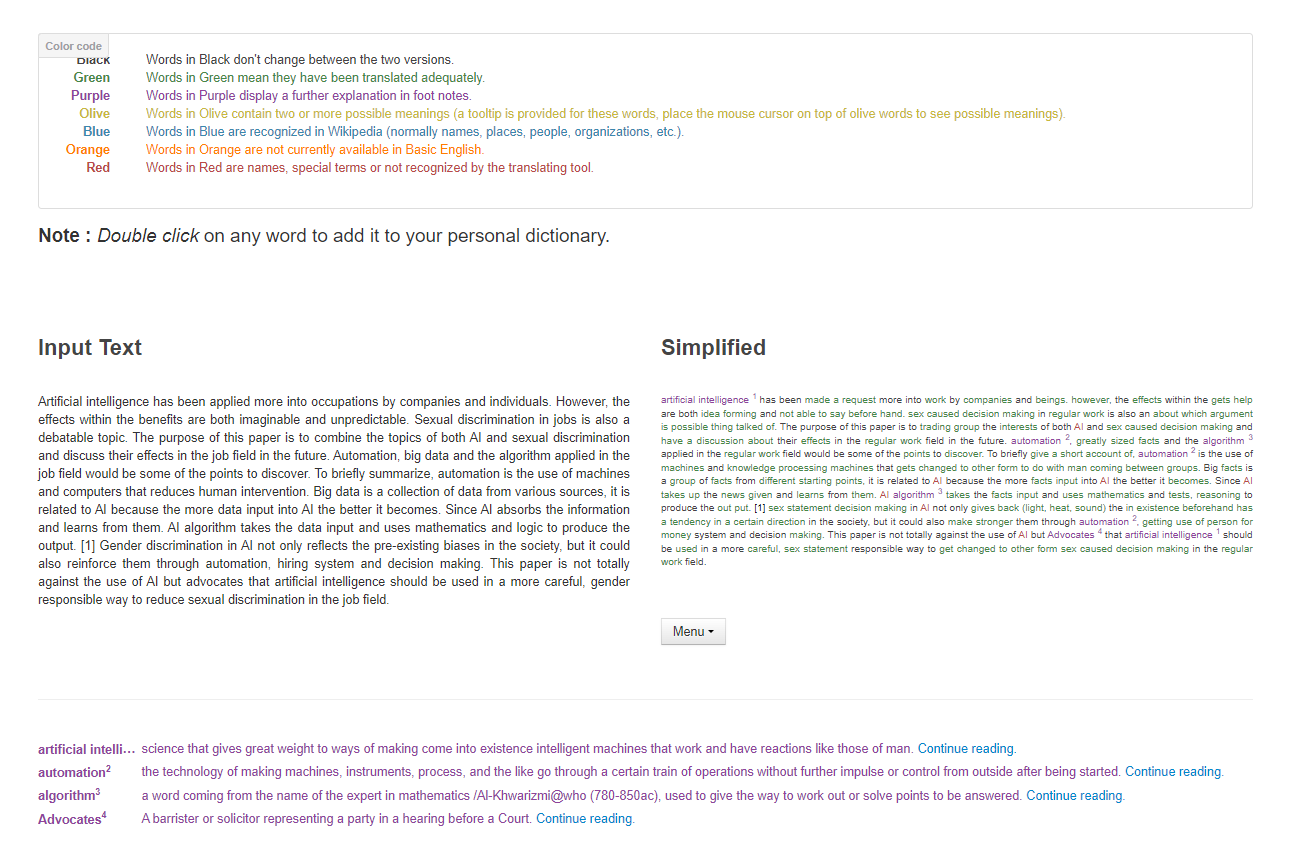
\includegraphics[width=\linewidth]{img/simplish-output.png}
	\label{img:simplish-output}
\end{figure}

Bespreking van de Moscow

\begin{center}
	\begin{tabular}{ | m{4cm} | m{12cm} | } 
		\hline
		\textbf{MoSCoW-principe} & Functionaliteit \\
		\hline
		Must-have & Gepersonaliseerde vereenvoudiging aanbieden, waaronder lexicale en syntactische vereenvoudiging aanbieden, na het toevoegen van een respectievelijke API-sleutel. \\
		& Wetenschappelijke artikelen in PDF-vorm opladen. \\
		& Personaliseerbare site: lettertype -en grootte aanpassen, tekstformaat aanpassen, achtergrondkleur aanpassen \\
		& Lokale opzet \\
		\hline
		Should-have & Glossary genereren na handmatige selectie van moeilijke woorden \\
		& Personaliseerbare PDF- of Worddocumentlay-out \\
		& Uitvoer als PDF of Word-bestand teruggeven. \\
		& Tekstanalyse voor en na de vereenvoudiging aanbieden. \\
		\hline
		Could-have & Glossary genereren na automatische selectie van moeilijke woorden \\
		\hline
		Wont-have & Beschikbaarheid tot de tool zonder Docker Desktop, in de vorm van online webtoepassing of browserextensie. \\
		& Beschikbaarheid tot de standaard- en gepersonaliseerde opties zonder API-sleutels \\
		\hline
	\end{tabular}
\end{center}

% 3. Beperkingen bespreken

De requirementsanalyse neemt geen functionaliteiten op van obscure proof-of-concepten. Deze ontbreken de nodige testen en zekerheid dat deze effectieve gepersonaliseerde en geautomatiseerde tekstvereenvoudiging aanbieden. Twee van de online tools, namelijk Resoomer en Scispace, bieden uitsluitend samenvattingsfunctionaliteiten aan. Resoomer is sneller geneigd om de belangrijkste zinnen te markeren en vervolgens deze in een kortere tekst terug te geven. Dit kan een effect hebben op de betrouwbaarheid van de functionaliteiten, alsook op de leesgraadmetrieken.

% 4. Implicaties aanduiden

% Wat voor gevolgen heeft jouw onderzoek?

% Wat gebeurt mogelijk in de toekomst wanneer de huidige situatie niet verandert (waarover jij een conclusie hebt getrokken)? In andere woorden, wat zijn de gevolgen als er geen oplossing wordt gevonden of doorgevoerd?

% 5. Suggesties voor vervolgonderzoek geven


\section{Vergelijkende studie}

% Taalmodel 1: ...
% Taalmodel 2: ...
% Taalmodel 3: ...
% Taalmodel 4: GPT-3

De huidige softwaretools die worden gebruikt in het middelbaar onderwijs zijn niet in staat om de oorspronkelijke tekst te transformeren, wat betekent dat syntactische vereenvoudiging momenteel niet haalbaar is. Hoewel er online webtoepassingen beschikbaar zijn, bieden ze minder functionaliteiten om de moeilijkheidsgraad van zinsyntaxis te verlagen en zijn ze voornamelijk gericht op het verkorten van de oorspronkelijke tekst ofwel samenvatting. Het aanpassen van tangconstructies, verwijswoorden, voorzetseluitdrukkingen, samengestelde werkwoorden en onregelmatige werkwoorden blijft daarom een uitdaging voor deze toepassingen. Zelfs het schrijven in de actieve stem kan problematisch zijn, en er zijn alleen vooraf gedefinieerde prompts beschikbaar om deze transformaties uit te voeren.

\medspace

HuggingFace-taalmodellen zijn zoals verwezen in de bijlage, minder in staat om syntactische vereenvoudiging op een tekst toe te passen. De twee uitgeteste taalmodellen zijn voornamelijk gebouwd om lexicale vereenvoudiging te realiseren.

Hoewel taalmodellen zoals T4 in staat zijn om zinsyntaxtransformaties uit te voeren, kunnen ze problemen ondervinden bij het verwerken van alle meegegeven transformaties. Het taalmodel kan transformaties ontbreken als alle transformaties in één prompt zijn betrokken. De voorgestelde aanpak hiervoor bestaat uit een pipeline van minstens drie transformaties ofwel drie prompts. 

\medspace

Ontwikkelaars kunnen voor lexicale vereenvoudigingstaken gebruik maken van algemene taalmodellen die vrij beschikbaar staan op \textit{HuggingFace}. Deze taalmodellen komen te kort bij gepersonaliseerde tekstvereenvoudigingstaken en daarom kunnen ontwikkelaars GPT-3 inschakelen als taalmodel voor gepersonaliseerde tekstvereenvoudiging van wetenschappelijke artikelen. Het uitgeteste GPT-3-model blinkt uit in gepersonaliseerde vereenvoudigingstaken. Engelstalige prompts die expliciet de uitvoertaal vermelden zijn nauwkeuriger dan Nederlandstalige prompts. Geen enkel taalmodel kan gegarandeerd rekening houden met de doelgroep. GPT-3 komt dichtbij, maar maakt enkele inschattingsfouten.

\section{Opbouw van het prototype}

API's toepassen in een prototype verlaagt de gebruikte geheugenruimte en vermindert de benodigde rekenkracht van het systeem waarop het prototype draait. Eenmaal ontwikkelaars de toepassing willen uitrollen naar het grote publiek, kunnen zij gebruik maken van lokaal gehoste taalmodellen in plaats van taalmodellen per API. AI-ontwikkelaars kunnen de taalmodellen verder finetunen en trainen op nog meer datasets en daarmee kunnen zij betere resultaten krijgen.

Intuïtieve handelingen kunnen vrij snel en eenduidig worden ontwikkeld door middel van HTML en JavaScript. Er is geen complex framework nodig om deze handelingen te kunnen ontwikkelen, alsook is de kennis sporadisch online beschikbaar. Sites en webontwikkelaars houden zelden rekening met deze personalisatiemogelijkheden, al wijst dit onderzoeksdeel uit dat deze methoden eenvoudig te ontwikkelen zijn voor pas afgestudeerde bachelorstudenten. AI-softwarebedrijven moeten meer inzetten op de personalisatie-opties voor scholieren met dyslexie in de derde graad van het middelbaar onderwijs, die momenteel het meest betrokken zijn in de digitalisering.
